\documentclass[12pt]{article}
\usepackage{amssymb,latexsym,amsmath}

\newif\ifpdf
\ifx\pdfoutput\undefined
\pdffalse % we are not running PDFLaTeX                                         
\else
\pdfoutput=1 % we are running PDFLaTeX                                          
\pdftrue
\fi
\ifpdf
\usepackage[pdftex]{graphicx}
\else
\usepackage{graphicx}
\fi
\ifpdf
\DeclareGraphicsExtensions{.pdf, .jpg, .tif}
\else
\DeclareGraphicsExtensions{.eps, .jpg}
\fi



\textwidth = 6.5 in
\textheight = 9 in
\oddsidemargin = 0.0 in
\evensidemargin = 0.0 in
\topmargin = 0.0 in
\headheight = 0.0 in
\headsep = 0.0 in
\parskip = 0.2 in
\parindent = 0.0 in


%%%%%%%%%%%%%%%%%%%%%%%%%%%%%%%%%%%%%%%%%%%%%%%%%%%%%%%%%%%%%%%%%%%%%%%%


\newcommand{\khat}{\hat{\mathbf k}}
\newcommand{\uv}{\mathbf u}
\newcommand{\up}{\mathbf u'}
\newcommand{\w}{\mathbf w}
\newcommand{\grad}{\nabla}
\newcommand{\curlp}{\gradp \times}
\newcommand{\curl}{\grad \times}
\newcommand{\gradp}{\nabla'}

\DeclareMathOperator{\Span}{span}


\title{Coordinate scaling in the LANL DNS code}
\author{Mark Taylor}

\begin{document}
%\maketitle

\section{Scaling of the Domain}
\begin{figure}
\begin{center}
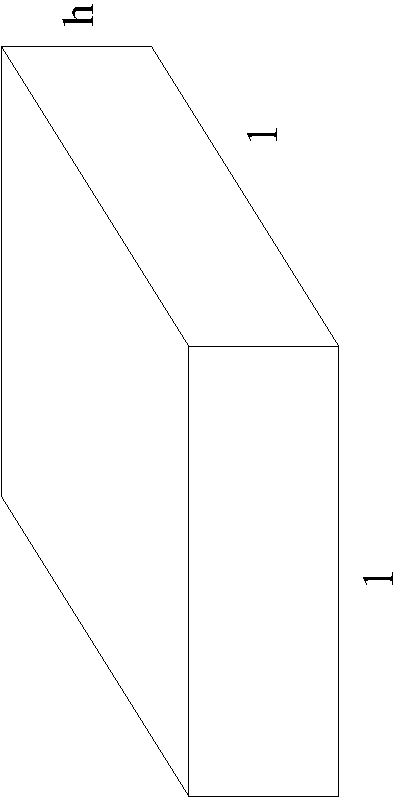
\includegraphics[angle=-90,width=4in]{box}
\caption{ }
\label{F:box}
\end{center}
\end{figure}



We would like to solve the NS equations in the box pictured in
Fig.~\ref{F:box}.  To write the equations in this domain, we use
primes:
\[
\frac{ \partial  \up }{\partial t}  + (\curlp \up + f \khat) \times \up + \gradp \pi' = \nu \Delta' \up
\]
\[
\gradp \cdot \up = 0
\]
with
\[
\gradp = 
\begin{pmatrix} \dfrac{\partial}{\partial x'} \\[5mm]
                \dfrac{\partial}{\partial y'} \\[5mm]
                \dfrac{\partial}{\partial z'} 
\end{pmatrix}
 \qquad
\Delta'  = \left(\frac{\partial}{\partial x'}\right)^2 + 
           \left(\frac{\partial^2}{\partial y'}\right)^2 +
           \left(\frac{\partial^2}{\partial z'}\right)^2 
\]
We now introduce a change of variables, into the {\em non-primed} coordiante
system.  In the non-primed coordinate system, the domain because a 
unit cube:
\[
x = x', \qquad y=y', \qquad  z = \frac{z'}{L}
\]
and
\[
u_1 = u_1', \qquad u_2 = u_2', \qquad  L u_3 = u_3'
\]
And we also have:
\[
\frac{\partial}{\partial z'} = \frac{1}{L} \frac{\partial}{\partial z}
\]
We first write $\gradp \cdot \up$ in the non-primed coordinate system:
\[
\frac{\partial u_1' }{\partial x'} = \frac{\partial u_1 }{\partial x}
\qquad
\frac{\partial u_2' }{\partial y'} = \frac{\partial u_2 }{\partial y}
\qquad
\frac{\partial u_3' }{\partial z'} = \frac{1}{L} \frac{\partial L u_3 }{\partial z}
= \frac{\partial u_3 }{\partial z}
\]
So we have that
\[
\gradp \cdot \up = \grad \cdot \uv
\]
And thus the divergence free condition is the 
same in both coordinate systems.  The term $\gradp \pi'$ is the
unique gradient which maintains $\gradp \cdot \up = 0$, so in the
non-primed coordiante systems we can write this term as 
$\grad \pi$, where now it is the unique gradient which maintains 
$\grad \cdot \uv = 0$.
We now start substituting the non-primed variables with the
primted variables:
\[
\begin{pmatrix} u_1 \\
                u_2 \\
                L u_3 \\
\end{pmatrix}_t
  + (\curlp \up + f \khat) \times 
\begin{pmatrix} u_1 \\
                u_2 \\
                L u_3 \\
\end{pmatrix}
+ \grad \pi = \nu 
\begin{pmatrix} \dfrac{\partial^2 u_1}{\partial x^2} + 
                \dfrac{\partial^2 u_1}{\partial y^2} + 
                \dfrac{1}{L^2}\dfrac{\partial^2 u_1}{\partial z^2}   \\[5mm]
                \dfrac{\partial^2 u_2}{\partial x^2} + 
                \dfrac{\partial^2 u_2}{\partial y^2} + 
                \dfrac{1}{L^2}\dfrac{\partial^2 u_2}{\partial z^2}   \\[5mm]
                L \left( 
                \dfrac{\partial^2 u_3}{\partial x^2} + 
                \dfrac{\partial^2 u_3}{\partial y^2} + 
                \dfrac{1}{L^2}\dfrac{\partial^2 u_3}{\partial z^2} \right)
\end{pmatrix}
\]
Defining $\omega$ by  
\begin{equation}
\label{E:vor}
\omega = \curlp \up = 
\begin{pmatrix}
L \dfrac{\partial u_3}{\partial y} - \dfrac{1}{L} \dfrac{\partial u_2}{\partial z}  \\[5mm]
\dfrac{1}{L} \dfrac{\partial u_1}{\partial z} -  \dfrac{\partial u_3}{\partial x}  \\[5mm]
\dfrac{\partial u_2}{\partial x} - \dfrac{\partial u_1}{\partial y}
\end{pmatrix}  
\end{equation}
the vorticity term works out to 
\[
(\curlp \up + f\khat) \times 
\begin{pmatrix} u_1 \\
                u_2 \\
                L u_3 \\
\end{pmatrix} = 
\begin{pmatrix} L u_3 w_2 - u_2 w_3 \\
                u_1 w_3 - L u_3 w_1 \\
                u_2 w_1 - u_1 w_2 \\
\end{pmatrix}  
+ 
\begin{pmatrix} -f u_2 \\
                f u_1 \\
                0  \\
\end{pmatrix}  
\]
Thus the final equations, after scaling the $z$ component by $L$:
\[
\begin{pmatrix} u_1 \\
                u_2 \\
                u_3 \\
\end{pmatrix}_t
  + 
\begin{pmatrix} L u_3 w_2 - u_2 w_3 \\
                u_1 w_3 - L u_3 w_1 \\
                \dfrac{1}{L} (u_2 w_1 - u_1 w_2) \\
\end{pmatrix}  
+ 
\begin{pmatrix} -f u_2 \\
                f u_1 \\
                0  \\
\end{pmatrix}  
+ \grad \pi = \nu 
\begin{pmatrix} \dfrac{\partial^2 u_1}{\partial x^2} + 
                \dfrac{\partial^2 u_1}{\partial y^2} + 
                \dfrac{1}{L^2}\dfrac{\partial^2 u_1}{\partial z^2}   \\[5mm]
                \dfrac{\partial^2 u_2}{\partial x^2} + 
                \dfrac{\partial^2 u_2}{\partial y^2} + 
                \dfrac{1}{L^2}\dfrac{\partial^2 u_2}{\partial z^2}   \\[5mm]
                \dfrac{\partial^2 u_3}{\partial x^2} + 
                \dfrac{\partial^2 u_3}{\partial y^2} + 
                \dfrac{1}{L^2}\dfrac{\partial^2 u_3}{\partial z^2}
\end{pmatrix}
\]
\newpage
Thus the only changes needed for our parallel DNS code are:
\begin{enumerate}
\item initial velocity given in the $\up$ coordinate system 
needs to be scaled to the non-primed coordinate system $\uv$.
\item Our output files will contain velocity will be in the non-primed 
$\uv$ coordinate system.  Need to scaled appropriately  to be analysed
by other codes.  Need to add a new output file header type that
contains L.  
\item modify computation of vorticity to match Eq.~\ref{E:vor}.
\item modify Laplacian (scale $z$ derivative terms by $1/L^2$).
\item modify vorticity term $\w \times \uv$ as shown above.
\end{enumerate}



\section{Computing 3D Energy Spectra (in a spherical shell)}
We would like to discretize our domain so that the 
maximum wave number (in the primed coordinate system) is
the same in all diretions.  Equivalently
\[
\Delta x' = \Delta y' = \Delta z'
\]
Or
\[
N_x  = N_y = N_z/L
\]
where $N_x$ is the number of grid points in the $x$ direction.
The highest wave number is given by:
\[
k_x = \pi N_x, \qquad k_y = \pi N_y, \qquad k_z = \pi N_z/L 
\]
(Note that $\pi$ appears in the wave numbers since our domain is
of length 1 in the $x$ and $y$ diretions.)  The wave number spacing
is given by
\[
\Delta k_x = 2 \pi, \qquad  \Delta k_y = 2 \pi, \qquad  \Delta k_z = 2 \pi / L 
\]
In our DNS code, we index our arrays of Fourier coefficients
with integers $(l,m,n)$, with $l=0 \dots N_x/2$, 
$m=0 \dots N_y/2$ and 
$n=0 \dots N_z/2$.  The wave number spacing is given by
given by
\[
k_x = l \Delta k_x,, \qquad  k_y = m \Delta k_y, \qquad  k_z = n  \Delta k_z
\]
We index the arrays containing power spectra
such as $E(k)$ with integer wave number $k$, represents a shell or anulus
of some chosen thickness centered around the wave number associated
with $k$.

The total energy is
\[
E  = \sum_{l,m,n}  |  {\hat u_1}(l,m,n) |^2 +
 |  {\hat u_2}(l,m,n) |^2 + 
 |  L {\hat u_3}(l,m,n) |^2
\]

The standard energy spectrum is now, for integers $k$:
\[
E(k)  = \sum_{l,m,n}  |  {\hat u_1}(l,m,n) |^2 +
 |  {\hat u_2}(l,m,n) |^2 + 
 |  L {\hat u_3}(l,m,n) |^2
\]
where the sum is taken over all integers $(l,m,n)$ such that
\[
(\Delta k_z)^2 (k-1/2)^2 < (\Delta k_x l)^2 + (\Delta k_y m)^2 + (\Delta k_z n)^2 <  (\Delta k_z)^2 (k+1/2)^2 
\]
where we have chosen to use a shell thickness of $\Delta k_z$.
 Scaling out the $2\pi$, we get
\[
\frac{(k-1/2)^2}{L^2} < l^2 + m^2 + \frac{n^2}{L^2} < \frac{(k+1/2)^2}{L^2}
\]  




\section{Computing 2D Energy Spectra (in an annulus)}
There are two different 2D spectra we need to compute. 
\begin{eqnarray}
E_0(k_h) &=& E(k_h, k_z=0) 
\label{E:SPECa} \\
E(k_h) &=& \sum_{k_z=0}^{\pi N_z/L} E(k_h,k_z) 
\label{E:SPECb}
\end{eqnarray}
where $k_h = \sqrt{(k_x^2 + k_y^2)} = \sqrt{(2\pi l)^2 + (2\pi m)^2}$. 
Eq.~\ref{E:SPECa} represents the energy spectrum of the 2D field
obtained by averaging the original 3D field  in the direction of rotation,
and then summing the energy within spherical shells (an annulus for 2D fields).  
Eq.~\ref{E:SPECb} represents
the energy spectrum of the full 3D field, but instead of 
summing the energy within spherical shells in wave number space, the sum is
taken over the annular region between concentric cylinders
(whose axis are in the $z$ direction).  As with the spherical
shell spectrum, Eq.~\ref{E:SPECb} has the property that
it partitions the energy into a set of discrete wave numbers, so
that the total energy 
\[
E = \sum_{k_h} E(k_h)
\]


The 2D shell (annulus) thickness is now
determined by the horizontal wavenumber spacings. In our code,
we use an integer index $k$ defined by $k_h = k \Delta k_x$ and
define
\begin{eqnarray*}
E_0(k) = \sum_{l,m}  |  {\hat u_1}(l,m,n=0) |^2 +
 |  {\hat u_2}(l,m,n=0) |^2 + 
 |  L {\hat u_3}(l,m,n=0) |^2
\end{eqnarray*}
where the sum is taken over all integers $(l,m)$ such that $n=0$ and
\[
(\Delta k_x)^2 (k-1/2)^2 < (\Delta k_x l)^2 + (\Delta k_y m)^2  <  (\Delta k_x)^2 (k+1/2)^2 
\]
and with $k_x=k \Delta k_x$ for integers $k$.  
we have chosen to use a shell thickness of $\Delta k_x = \Delta
k_y = 2\pi$. Scaling out the $2\pi$, we get
\[
(k-1/2)^2 < l^2 + m^2 < (k+1/2)^2.
\]  

The second spectrum is computed the same way as above except that now
we sum over all wave numbers $n$ for a given 2D shell:
\begin{eqnarray}
E(k) = \sum_{n=0}^{N_z/2} \sum_{l,m} |  {\hat u_1}(l,m,n) |^2 +
 |  {\hat u_2}(l,m,n) |^2 + 
 |  L {\hat u_3}(l,m,n) |^2
\end{eqnarray}
where for each $n$ the contribution to the shell $k_h$ is 
taken over all integers $(l,m)$ such that
\[
(k-1/2)^2 < l^2 + m^2 < (k+1/2)^2.
\]  



\end{document}